\section{Évaluation expérimentale}
\label{sec:evaluation-experimentale}
\label{sec:exp}
\label{sec:experiments}

\subsection{Protocole et classes de preuve}

L'évaluation distingue strictement trois classes de preuves.
Premièrement, la trace instrumentée end-to-end canonique Q1--Q6 et
les campagnes A, B et C établissent le comportement opérationnel du
prototype et, lorsque cela est explicitement observé, le contrat
d'exécution physique. Deuxièmement, les campagnes contrôlées de
sensibilité évaluent des facteurs déclarés sur des charges communes
et selon des protocoles préenregistrés. Troisièmement, les analyses de
précision portent sur la latence de décision sémantique et ne doivent
pas être interprétées comme des mesures de latence du backend.

Aucune métrique fondée sur des annotations humaines ou expertes
(precision, recall, F1 ou $\kappa$) n'est rapportée ici, faute de
provenance canonique d'annotation permettant de soutenir ce type
d'inférence. Les requêtes Q1--Q6 constituent une seule trace
séquentielle de six étapes et ne sont donc pas traitées comme six
observations indépendantes.

\subsection{Trace canonique Q1--Q6}

La trace Q1--Q6 est exécutée sur AdventureWorksDW via l'adaptateur
SQL Server Direct. Les trois premières requêtes apportent
successivement les exigences SalesAmount, TotalProductCost et
GrossMargin. La progression cumulative de l'objectif vaut donc
$1/3$, $2/3$ puis $1$. Ces trois requêtes sont autorisées et atteignent
l'exécution physique.

Les trois étapes suivantes illustrent le fait que la satisfaisabilité
formelle ne suffit pas à autoriser une requête. Q4 est satisfaisable
mais hors du périmètre de l'objectif et est bloquée avant backend. Q5
est bloquée pour incompatibilité de granularité. Q6 est satisfaisable
et réalise intrinsèquement une exigence déjà présente, mais sa
contribution marginale est nulle; elle est donc bloquée comme
redondante. Au total, la trace contient trois ALLOW et trois BLOCK,
avec trois exécutions physiques et trois arrêts avant backend.

\subsection{Campagnes opérationnelles A, B et C}

La Campagne A constitue l'évaluation de profondeur sur FoodMart. Le
bloc consolidé comprend 1000 sessions et 7960 décisions: 2266 ALLOW
et 5694 BLOCK. Toutes les décisions ALLOW ont donné lieu à une
exécution physique, alors que tous les BLOCK ont été stoppés avant
backend. Les 2266 ALLOW ont également produit 2266 mises à jour CKG
utiles. Aucune violation du contrat d'exécution physique n'a été
observée dans ce périmètre.

La Campagne B étend ce contrat à trois scénarios contrôlés couvrant
FoodMart via XMLA/Mondrian, AdventureWorks via SQL Direct et
SteelWheels via SQL Direct. Les 18 requêtes donnent 7 ALLOW et
11 BLOCK, soit 7 exécutions physiques et 11 arrêts avant backend.
Cette campagne documente donc la portabilité observée du contrat
d'exécution physique sur les entrepôts et adaptateurs testés, sans
revendiquer une invariance universelle.

La Campagne C compare, pour AdventureWorks, les mêmes six requêtes
logiques sous SQL Direct et XMLA/eMondrian. Il s'agit de douze
évaluations mais de six requêtes logiques appariées. Les deux
conditions conservent les mêmes identifiants, le même ordre, les
mêmes décisions, les mêmes raisons et la même politique d'exécution
physique. Cette observation soutient la préservation du contrat de
décision sur ce scénario contrôlé; elle ne constitue ni une preuve
d'invariance globale entre backends ni une comparaison de leurs
performances.

\begin{table*}[t]
\centering
\caption{Synthèse des preuves expérimentales canoniques retenues pour l'article.}
\label{tab:experimental-evidence-final}
\small
\begin{tabular}{p{0.18\textwidth}p{0.18\textwidth}p{0.19\textwidth}p{0.35\textwidth}}
\hline
Bloc & Volume & Exécution physique & Résultat principal \\
\hline
Trace Q1--Q6
& 6 requêtes, une trace instrumentée
& 3 ALLOW exécutées, 3 BLOCK stoppées avant backend
& Progression cumulative de l'objectif de $1/3$ à $1$; Q4 hors périmètre, Q5 granularité incompatible, Q6 redondante. \\

Campagne A
& 1000 sessions, 7960 décisions
& 2266 exécutions physiques; 5694 BLOCK avant backend
& 2266 ALLOW, 5694 BLOCK, zéro violation du contrat d'exécution physique et 2266 mises à jour CKG utiles. \\

Campagne B
& 3 scénarios, 18 requêtes
& 7 exécutions physiques; 11 arrêts avant backend
& Validation du contrat d'exécution physique sur FoodMart/XMLA, AdventureWorks/SQL Direct et SteelWheels/SQL Direct dans le périmètre testé. \\

Campagne C
& 6 requêtes logiques appariées, 12 évaluations
& 4 exécutions physiques; 8 BLOCK
& Même ordre, mêmes décisions, mêmes raisons et même politique physique entre SQL Direct et XMLA/eMondrian sur le scénario AdventureWorks contrôlé. \\
\hline
\end{tabular}
\end{table*}


\subsection{Robustesse contrôlée, comparaison principale et ablations}

La comparaison principale aux politiques de référence est fondée sur le
\emph{freeze} canonique de robustesse, et non sur les anciens rebuilds de mai.
Cette campagne est gelée pour les résultats non temporels; aucune affirmation
de latence n'en est dérivée. Elle couvre les politiques de référence et les
ablations principales sous un protocole commun, ce qui évite de traiter les
replays de versions antérieures comme des réplications indépendantes.

\begin{table*}[t]
\centering
\caption{Robustesse contrôlée : synthèse non temporelle des politiques adoptées.}
\label{tab:v3-robustness-main}
\small
\begin{tabular}{p{0.23\textwidth}p{0.09\textwidth}p{0.10\textwidth}p{0.11\textwidth}p{0.11\textwidth}p{0.16\textwidth}}
\hline
Politique & Sessions & Phi final & False ALLOW & False BLOCK & Exec. non contributive \\
\hline
mcad & 240 & 0.5 & 0.0 & 0.0 & 0.0 \\
baseline\_naive & 240 & 0.5 & 0.752083 & 0.0 & 0.752083 \\
baseline\_measure\_overlap & 240 & 0.5 & 0.660417 & 0.0 & 0.73125 \\
baseline\_random\_matched & 240 & 0.119444 & 0.211597 & 0.185833 & 0.650556 \\
ablation\_no\_sat & 240 & 0.5 & 0.041667 & 0.0 & 0.125 \\
ablation\_no\_real & 240 & 0.5 & 0.08125 & 0.0 & 0.1875 \\
ablation\_ceval\_any\_intersection & 240 & 0.5 & 0.08125 & 0.0 & 0.1875 \\
\hline
\end{tabular}
\end{table*}


\begin{figure}[t]
\centering
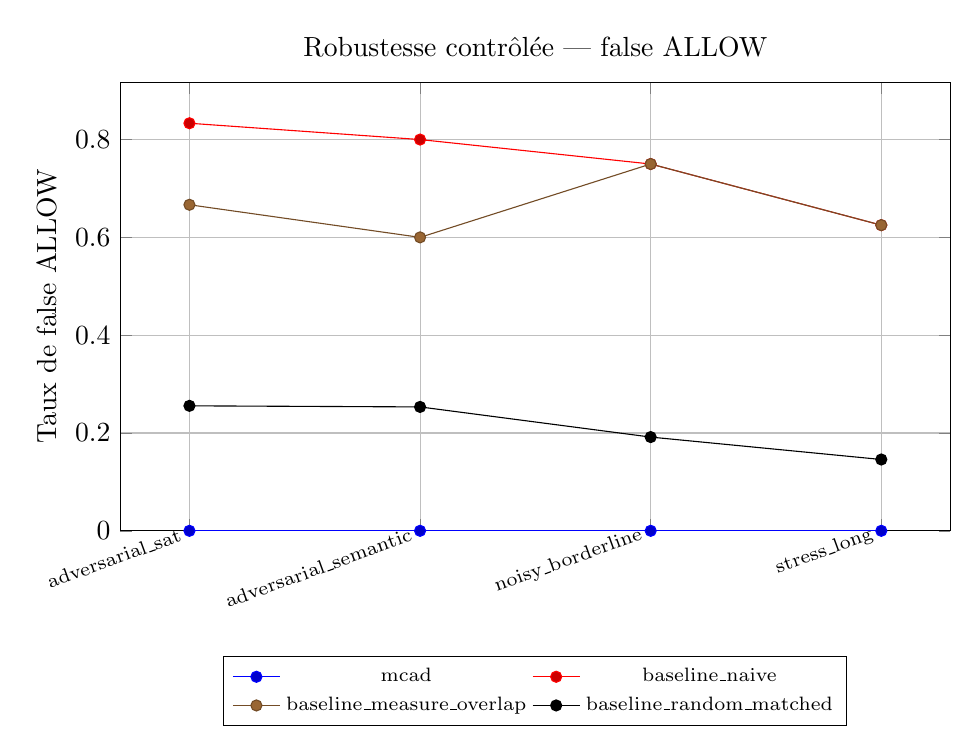
\begin{tikzpicture}
\begin{axis}[width=\linewidth,
height=0.60\linewidth,
title={Robustesse contrôlée — false ALLOW},
ylabel={Taux de false ALLOW},
xtick={0,1,2,3},
xticklabels={{adversarial\_sat},{adversarial\_semantic},{noisy\_borderline},{stress\_long}},
x tick label style={rotate=20,anchor=east,font=\scriptsize},
grid=major,
legend style={font=\scriptsize,at={(0.5,-0.28)},anchor=north,legend columns=2},
ymin=0]
\addplot+[mark=*] coordinates {(0,0.0) (1,0.0) (2,0.0) (3,0.0)};
\addlegendentry{mcad}
\addplot+[mark=*] coordinates {(0,0.833333) (1,0.8) (2,0.75) (3,0.625)};
\addlegendentry{baseline\_naive}
\addplot+[mark=*] coordinates {(0,0.666667) (1,0.6) (2,0.75) (3,0.625)};
\addlegendentry{baseline\_measure\_overlap}
\addplot+[mark=*] coordinates {(0,0.255556) (1,0.253333) (2,0.191667) (3,0.145833)};
\addlegendentry{baseline\_random\_matched}
\end{axis}
\end{tikzpicture}

\caption{Taux de \emph{false ALLOW} dans les familles de scénarios du freeze de robustesse.}
\label{fig:v3-robustness-false-allow}
\end{figure}

Les BLOCK de MCAD disposent d'une explication système fondée sur les clauses
échouées et/ou les exigences manquantes. Cette propriété ne constitue pas une
validation de compréhension par des experts humains.

\begin{figure}[t]
\centering
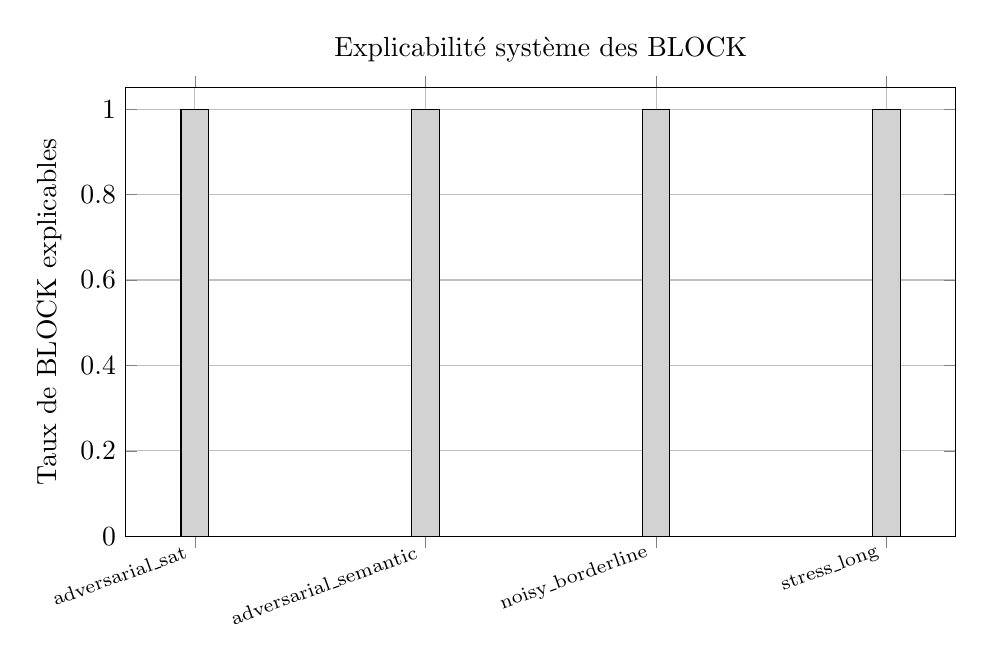
\begin{tikzpicture}
\begin{axis}[ybar,
bar width=10pt,
width=\linewidth,
height=0.60\linewidth,
title={Explicabilité système des BLOCK},
ylabel={Taux de BLOCK explicables},
xtick={0,1,2,3},
xticklabels={{adversarial\_sat},{adversarial\_semantic},{noisy\_borderline},{stress\_long}},
x tick label style={rotate=20,anchor=east,font=\scriptsize},
ymin=0,
grid=major,
ymax=1.05]
\addplot+[draw=black,fill=gray!35] coordinates {(0,1.0) (1,1.0) (2,1.0) (3,1.0)};
\end{axis}
\end{tikzpicture}

\caption{Explicabilité système des BLOCK dans le freeze de robustesse.}
\label{fig:v3-robustness-explainability}
\end{figure}

\subsection{Scalabilité structurelle du CKG}

La scalabilité est mobilisée uniquement au sens structurel. Le runner
historique qualifié est byte-identique au runner courant et les entrées
historiques n'activent pas l'extension \texttt{session\_support\_policy}
introduite pour \texttt{objective\_count} v2. Les timings historiques de mai
sont exclus.

\begin{table*}[t]
\centering
\caption{Scalabilité structurelle du CKG sur les échelles qualifiées.}
\label{tab:v3-scalability-structural}
\small
\begin{tabular}{p{0.08\textwidth}p{0.10\textwidth}p{0.11\textwidth}p{0.08\textwidth}p{0.09\textwidth}p{0.09\textwidth}p{0.18\textwidth}}
\hline
Échelle & Objectifs & Contraintes & NV & Nœuds & Arêtes & Snapshot (octets) \\
\hline
1 & 3 & 8 & 10 & 55 & 66 & 43501 \\
5 & 11 & 32 & 42 & 223 & 306 & 207117 \\
10 & 21 & 62 & 82 & 433 & 606 & 412597 \\
20 & 41 & 122 & 162 & 853 & 1206 & 822597 \\
40 & 81 & 242 & 322 & 1693 & 2406 & 1642597 \\
\hline
\end{tabular}
\end{table*}


\begin{figure}[t]
\centering
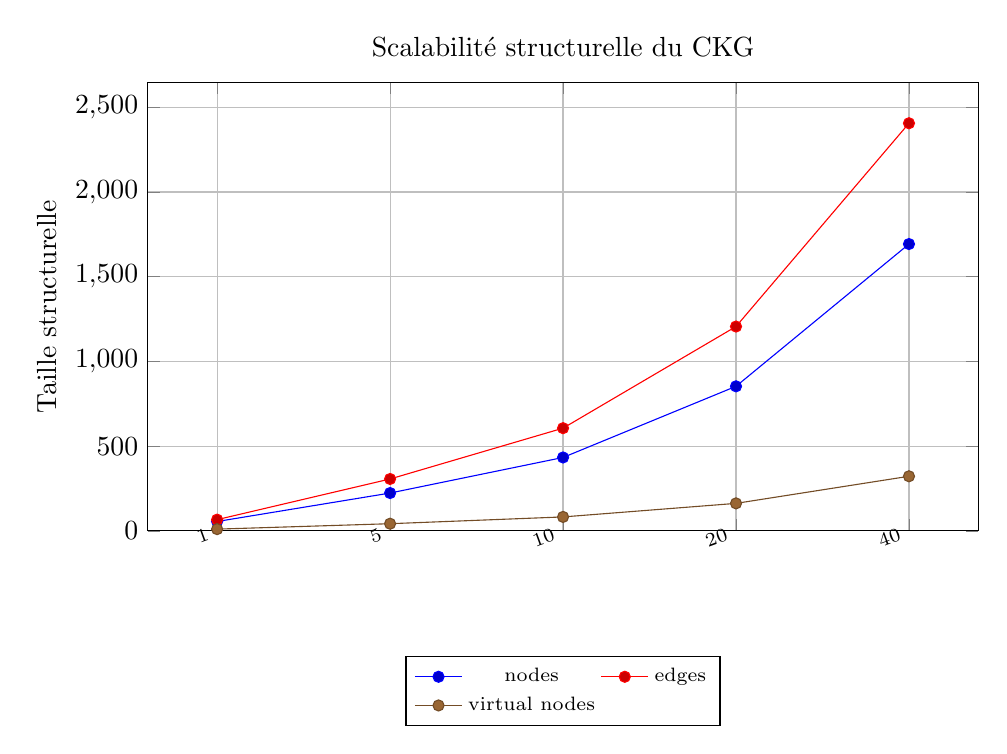
\begin{tikzpicture}
\begin{axis}[width=\linewidth,
height=0.60\linewidth,
title={Scalabilité structurelle du CKG},
ylabel={Taille structurelle},
xtick={0,1,2,3,4},
xticklabels={{1},{5},{10},{20},{40}},
x tick label style={rotate=20,anchor=east,font=\scriptsize},
grid=major,
legend style={font=\scriptsize,at={(0.5,-0.28)},anchor=north,legend columns=2},
ymin=0]
\addplot+[mark=*] coordinates {(0,55) (1,223) (2,433) (3,853) (4,1693)};
\addlegendentry{nodes}
\addplot+[mark=*] coordinates {(0,66) (1,306) (2,606) (3,1206) (4,2406)};
\addlegendentry{edges}
\addplot+[mark=*] coordinates {(0,10) (1,42) (2,82) (3,162) (4,322)};
\addlegendentry{virtual nodes}
\end{axis}
\end{tikzpicture}

\caption{Croissance structurelle du CKG aux facteurs d'échelle testés.}
\label{fig:v3-scalability-structure}
\end{figure}

\subsection{Utilité contrôlée de l'évidence}

Le benchmark Phase~6 d'utilité de l'évidence est conservé comme preuve secondaire compacte parce qu'il évalue une propriété distincte de la robustesse et de la scalabilité : la réutilisation d'une évidence persistée pour amorcer une session ultérieure. Dans ce protocole contrôlé, cette observation ne constitue ni une validation utilisateur ni une preuve de généralisation industrielle.

\begin{table*}[t]
\centering
\caption{Réutilisation contrôlée de l'évidence, preuve secondaire.}
\label{tab:v3-secondary-evidence}
\small
\begin{tabular}{p{0.21\textwidth}p{0.15\textwidth}p{0.12\textwidth}p{0.10\textwidth}p{0.10\textwidth}p{0.12\textwidth}}
\hline
Objectif & Mode & Étapes vers 1 & AUC & Phi final & Phi bootstrap \\
\hline
OHF\_NORD & no\_bootstrap & 3 & 0.666667 & 1.0 & 0.0 \\
OHF\_NORD & bootstrap & 1 & 1.0 & 1.0 & 0.666667 \\
OAW\_BIKES\_EUROPE & no\_bootstrap & 3 & 0.666667 & 1.0 & 0.0 \\
OAW\_BIKES\_EUROPE & bootstrap & 1 & 1.0 & 1.0 & 0.666667 \\
\hline
\end{tabular}
\end{table*}


\begin{table*}[t]
\centering
\caption{Bilan terminal des facteurs de sensibilité contrôlée.}
\label{tab:sensitivity-final}
\small
\begin{tabular}{p{0.21\textwidth}p{0.14\textwidth}p{0.55\textwidth}}
\hline
Facteur & Stade terminal retenu & Statut de publication \\
\hline
Nombre de contraintes
& Stage 20
& Campagne canonique Stage-20 gelée; les conclusions sont bornées au protocole et au freeze associés. \\

Nombre de noeuds virtuels
& Stage 10
& Cibles de précision préenregistrées atteintes au Stage-10; aucune extension Stage-20 requise. \\

Densité d'appartenance
& Stage 10
& Décision de précision Stage-10 PASS, selon l'artefact canonique sélectionné dans le source-map final. \\

Nombre d'objectifs
& Stage 30
& Limite terminale de précision: 17/192 cellules hors cibles préenregistrées après 30 clusters et 576000 mesures; aucun rerun, aucun bootstrap supplémentaire et aucun Stage-40. \\
\hline
\end{tabular}
\end{table*}


\subsection{Sensibilité et précision de la décision sémantique}

Les facteurs contrôlés retenus pour la publication sont le nombre de
contraintes, le nombre de noeuds virtuels, la densité d'appartenance
et le nombre d'objectifs. Leur source scientifique primaire est
figée par le source-map de publication associé au présent état du
dépôt.

Pour le nombre de noeuds virtuels, les cibles de précision
préenregistrées sont atteintes au Stage-10 et aucune extension
Stage-20 n'est requise. Pour la densité d'appartenance, la décision
canonique de précision au Stage-10 est PASS. Le nombre de contraintes
est rapporté depuis la campagne canonique Stage-20 gelée.

Le nombre d'objectifs requiert l'extension préenregistrée jusqu'au
Stage-30, stade maximal du protocole. L'analyse terminale porte sur
30 clusters structurels, 576000 mesures et 192 cellules
niveau--étape. Dix-sept cellules ne satisfont pas simultanément les
cibles de précision préenregistrées. Le statut terminal est donc
\texttt{stage30\_precision\_targets\_not\_met} et
\texttt{stage30\_sufficient=false}. Ce résultat n'est pas un échec
d'exécution: l'analyse canonique s'est terminée correctement et
constitue la limite de précision terminale prévue par le protocole.
Aucune réplication supplémentaire, aucun nouveau bootstrap et aucun
Stage-40 ne sont autorisés.

\subsection{Portée des conclusions}

Les résultats soutiennent, dans les scénarios étudiés, la distinction
entre satisfaisabilité, contribution à l'objectif et décision
d'autorisation, ainsi que l'application cohérente du gate physique:
un BLOCK est arrêté avant exécution backend alors qu'un ALLOW peut
atteindre l'adaptateur d'exécution. Les résultats de sensibilité
documentent la stabilité ou les limites de précision observées pour
les facteurs contrôlés.


La chaîne de preuve finale exclut explicitement les statistiques Phase~7
historiques de mai utilisées telles quelles, les mesures de latence des
rebuilds de mai, les anciennes figures proxy et les annotations
\texttt{sim\_expert}. Le benchmark nominal de mai et le benchmark Phase~6
d'utilité de l'évidence sont conservés comme preuves secondaires ou
supplémentaires et ne sont pas comptés comme réplications indépendantes du
freeze de robustesse.

Les statistiques Phase~7 historiques de mai ne sont pas utilisées telles quelles pour soutenir le freeze final de robustesse. Les latences des rebuilds de mai, les anciennes figures proxy, les annotations \texttt{sim\_expert} et les sorties intermédiaires/rejouées des sensibilités sont également exclues de la chaîne de preuve finale. Le benchmark nominal de mai reste uniquement supplémentaire.

Ces conclusions restent bornées au prototype, aux jeux de données,
aux scénarios, aux facteurs et aux protocoles expérimentaux
considérés. Elles ne démontrent ni supériorité universelle, ni
invariance générale vis-à-vis des backends, ni robustesse
industrielle hors du périmètre évalué.
